\documentclass[12pt]{standalone}
\usepackage{tikz}

\begin{document}
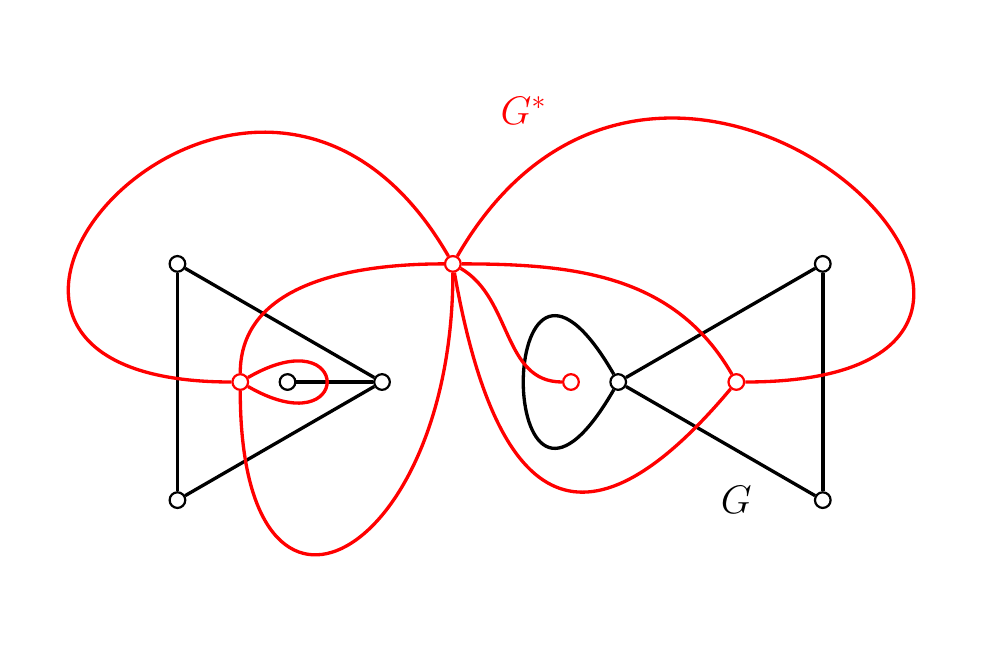
\begin{tikzpicture}[scale=1.5]
    \clip (-3,-2) rectangle (5,3);
    \node[circle, thick, draw, inner sep=2pt] (a) at (0,0) {};
    \node[circle, thick, draw, inner sep=2pt] (b) at (-1.732,-1) {};
    \node[circle, thick, draw, inner sep=2pt] (c) at (-1.732,+1) {};
    \node[circle, thick, draw, inner sep=2pt] (d) at (-0.8,0) {};
    \node[circle, thick, draw, inner sep=2pt] (e) at (2,0) {};
    \node[circle, thick, draw, inner sep=2pt] (f) at (3.732,-1) {};
    \node[circle, thick, draw, inner sep=2pt] (g) at (3.732,+1) {};
    \draw[very thick, black] (a) -- (b);
    \draw[very thick, black] (a) -- (c);
    \draw[very thick, black] (b) -- (c);
    \draw[very thick, black] (a) -- (d);
    \draw[very thick, black] (e) -- (f);
    \draw[very thick, black] (e) -- (g);
    \draw[very thick, black] (f) -- (g);
    \draw[very thick, black] (e) to[out=120,in=240,looseness=40] (e);
    \node[circle, thick, draw, inner sep=2pt, red] (A) at (0.6,1) {};
    \node[circle, thick, draw, inner sep=2pt, red] (B) at (-1.2,0) {};
    \node[circle, thick, draw, inner sep=2pt, red] (C) at (3,0) {};
    \node[circle, thick, draw, inner sep=2pt, red] (D) at (1.6,0) {};
    \draw[very thick, red, overlay] (A) to[out=120,in=180,looseness=4] (B);
    \draw[very thick, red, overlay] (A) to[out=180,in=90] (B);
    \draw[very thick, red, overlay] (A) to[out=270,in=270,looseness=3] (B);
    \draw[very thick, red, overlay] (B) to[out=30,in=330,looseness=35] (B);
    \draw[very thick, red, overlay] (A) to[out=280,in=230,looseness=2] (C);
    \draw[very thick, red, overlay] (A) to[out=0,in=120] (C);
    \draw[very thick, red, overlay] (A) to[out=60,in=0,looseness=3.5] (C);
    \draw[very thick, red, overlay] (A) to[out=330,in=180] (D);
    \node[red] at (1.2,2.3) {\Large $G^*$};
    \node[black] at (3,-1) {\Large $G$};
\end{tikzpicture}
\end{document}
